\documentclass[conference]{IEEEtran}
\IEEEoverridecommandlockouts
\usepackage{cite}
\usepackage{amsmath,amssymb,amsfonts}
\usepackage{algorithmic}
\usepackage{graphicx}
\usepackage{textcomp}
\usepackage{xcolor}
% Paquetes adicionales para el idioma, las tablas y el diagrama PRISMA
\usepackage[utf8]{inputenc}
\usepackage[T1]{fontenc}
\usepackage[spanish,es-noshorthands,es-tabla]{babel}
\usepackage{booktabs}
\usepackage{multirow}
\usepackage{array}
\usepackage{tikz}
\usetikzlibrary{positioning,arrows.meta,calc}
\usepackage{url}
\def\BibTeX{{\rm B\kern-.05em{\sc i\kern-.025em b}\kern-.08em
    T\kern-.1667em\lower.7ex\hbox{E}\kern-.125emX}}
\newcommand{\lnr}{\ln(\mathrm{RMSE}_{\mathrm{esp}}/\mathrm{RMSE}_{\mathrm{AA}})}
\renewcommand{\IEEEkeywordsname}{Palabras clave}
\begin{document}

\title{Metaanálisis del desempeño de la predicción espacial de variables ambientales mediante geoestadística y aprendizaje automático en regiones montañosas}

\author{\IEEEauthorblockN{Kris Ximena Colquehuanca Zapana}
\IEEEauthorblockA{\textit{Facultad de Ingeniería Estadística e Informática} \\
\textit{Universidad Nacional del Altiplano}\\
Puno, Perú}
\and
\IEEEauthorblockN{Yeferson Dariun Laura Livise}
\IEEEauthorblockA{\textit{Facultad de Ingeniería Estadística e Informática} \\
\textit{Universidad Nacional del Altiplano}\\
Puno, Perú}
\and
\IEEEauthorblockN{Obed Eliu Leon Mamani}
\IEEEauthorblockA{\textit{Facultad de Ingeniería Estadística e Informática} \\
\textit{Universidad Nacional del Altiplano}\\
Puno, Perú}
\and
\IEEEauthorblockN{Kevin Pleyer Portillo Machaca}
\IEEEauthorblockA{\textit{Facultad de Ingeniería Estadística e Informática} \\
\textit{Universidad Nacional del Altiplano}\\
Puno, Perú}
}

\maketitle

\begin{abstract}
En las regiones montañosas las redes de estaciones son escasas y se concentran en cotas bajas, mientras que la precipitación y la temperatura cambian con fuerza con el relieve. Para estimarlas en sitios sin medición se usan métodos geoestadísticos, que modelan la dependencia espacial, y algoritmos de aprendizaje automático (AA), pero la evidencia comparativa es contradictoria. Esta revisión sistemática, conducida según PRISMA 2020, sintetiza los estudios publicados entre 2020 y 2026 que comparan ambos enfoques en terreno montañoso con validación fuera de muestra frente a estaciones. De 263 registros de la búsqueda principal y 127 de una búsqueda complementaria, 18 estudios cumplieron los criterios de elegibilidad y 15 aportaron 16 comparaciones al metaanálisis. El efecto se expresó como el logaritmo de la razón entre el RMSE del método espacial y el del AA, y se combinó con un modelo de efectos aleatorios. En promedio, el AA redujo el RMSE en un 12,9 por ciento (intervalo de confianza del 95 por ciento: 4,5 a 20,6), con heterogeneidad moderada y un intervalo de predicción que incluye la ausencia de diferencia. La ventaja fue menor cuando ambos métodos usaron las mismas covariables, solo fue significativa con estaciones de validación independientes y desapareció en los tres estudios con bajo riesgo de sesgo. La evidencia procede sobre todo de China e Irán, solo un estudio corresponde a los Andes y ninguno al Altiplano. Los resultados sugieren una ventaja moderada pero frágil del AA, que depende de las covariables disponibles y del esquema de validación.
\end{abstract}

\begin{IEEEkeywords}
aprendizaje automático, geoestadística, kriging, metaanálisis, precipitación, regiones montañosas, random forest, temperatura del aire
\end{IEEEkeywords}

\section{Introducción}

Las montañas almacenan y regulan una fracción desproporcionada del agua dulce que consumen las poblaciones de las tierras bajas~\cite{viviroli2007}. Sin embargo, en ellas las redes de monitoreo meteorológico son escasas, están mal distribuidas y se concentran en los valles, justo donde la precipitación y la temperatura varían menos. Para producir mapas continuos que alimenten modelos hidrológicos, índices de sequía o planes de gestión del riesgo es necesario estimar estas variables en ubicaciones sin medición.

Dos familias de métodos dominan esta tarea. La geoestadística (kriging ordinario, universal o con deriva externa, regresión-kriging, cokriging) y las regresiones locales como la regresión geográficamente ponderada (GWR) modelan de forma explícita la dependencia espacial y han sido la referencia durante décadas~\cite{li2011}. El aprendizaje automático (AA), en particular random forest (RF), gradient boosting y las redes neuronales, aprende relaciones no lineales con covariables como la elevación o los productos satelitales y de reanálisis~\cite{appelhans2015,hengl2018}. En los últimos años han surgido además variantes de AA que incorporan explícitamente la información espacial~\cite{hengl2018,sekulic2020}.

La evidencia comparativa entre ambas familias es contradictoria: algunos estudios favorecen a los métodos con dependencia espacial y otros al AA. Las comparaciones están fragmentadas (pocos métodos en una sola cuenca, con métricas y esquemas de validación distintos) y la validación cruzada aleatoria puede sobrestimar el desempeño cuando los datos tienen estructura espacial~\cite{roberts2017,ploton2020}. Hasta donde sabemos, no existe una síntesis cuantitativa que compare el desempeño predictivo de ambos enfoques en regiones montañosas.

El objetivo de este trabajo es responder la siguiente pregunta: en regiones montañosas con redes de monitoreo escasas, ¿cómo se compara el desempeño predictivo fuera de muestra de la geoestadística frente al AA para estimar variables ambientales en ubicaciones sin medición, y qué factores explican las diferencias?

\section{Métodos}

\subsection{Protocolo y pregunta de investigación}
La revisión siguió la declaración PRISMA~2020~\cite{page2021}. La pregunta se estructuró con el esquema PICO. \emph{Población}: estudios primarios que estiman precipitación, temperatura del aire, índices de sequía (SPI, SPEI, VCI) o PM2.5 en ubicaciones sin medición, en regiones montañosas. \emph{Intervención}: métodos espaciales que modelan la dependencia espacial. \emph{Comparación}: algoritmos de AA con covariables equivalentes. \emph{Resultado}: desempeño predictivo fuera de muestra, medido principalmente como la razón logarítmica de RMSE. El protocolo no se registró de forma previa.

\subsection{Fuentes de información y búsqueda}
La búsqueda se realizó los días 12 y 13 de octubre de 2026 en Scopus, OpenAlex, SciELO y Redalyc; Web of Science no pudo consultarse por falta de acceso institucional. La ecuación canónica combinó con el operador AND cinco bloques de sinónimos unidos con OR: variable (\textit{precipitation, rainfall, ``air temperature'', ``drought index'', SPI, SPEI, VCI, ``PM2.5''}), contexto (\textit{mountain*, alpine, highland*, ``complex terrain'', Andes, Altiplano, Himalaya*, ``Tibetan Plateau''}), geoestadística (\textit{kriging, cokriging, geostatistic*, variogram, ``regression kriging'', ``geographically weighted regression''}), AA (\textit{``machine learning'', ``random forest'', XGBoost, ``gradient boosting'', ``support vector'', ``neural network*''}) y desempeño (\textit{RMSE, ``cross-validation'', ``predictive performance'', validation}). En SciELO y Redalyc se usaron los términos equivalentes en español y portugués. Se añadieron los estudios identificados en la búsqueda exploratoria del grupo. El 15 de octubre de 2026 se realizó una búsqueda complementaria en OpenAlex con seis ecuaciones adicionales, una de ellas específica para los Andes y el Altiplano, y un rastreo de citas hacia adelante y hacia atrás de los estudios incluidos; los registros nuevos se cribaron con los mismos criterios. Ese mismo día se hizo una búsqueda de verificación en Google Scholar con ocho consultas en inglés y español, limitadas a 2020--2026, revisando los primeros resultados de cada una (80 registros).

\subsection{Criterios de elegibilidad}
Un estudio se incluyó si cumplía los ocho criterios de inclusión (CI) y ninguno de los nueve de exclusión (CE) de la Tabla~\ref{tab:criterios}. La unidad de análisis fue la \emph{comparación}: un par método espacial--AA para una variable, un área y un esquema de validación.

\begin{table}[!t]
\caption{Criterios de elegibilidad}
\label{tab:criterios}
\centering
\footnotesize
\setlength{\tabcolsep}{3pt}
\begin{tabular}{@{}l p{7.4cm}@{}}
\toprule
\multicolumn{2}{@{}l}{\textbf{Inclusión (deben cumplirse todos)}}\\
CI1 & Artículo original revisado por pares, 2020--2026, en inglés, español o portugués.\\
CI2 & Precipitación, temperatura del aire, índice de sequía o PM2.5.\\
CI3 & Predicción espacial en sitios sin medición, validada con estaciones no usadas en el ajuste.\\
CI4 & Al menos un método espacial como brazo propio: KO, KU, KED, RK, STRK, CoK, EBK, GWR o MGWR.\\
CI5 & Al menos un método de AA como brazo propio: RF, GB, SVM, RNA, GPR o M5.\\
CI6 & Comparación directa en el mismo estudio: misma área, datos y validación.\\
CI7 & Área subnacional con relieve montañoso declarado o desnivel $\geq 1000$~m.\\
CI8 & Métrica de error para ambos brazos (RMSE de preferencia).\\
\midrule
\multicolumn{2}{@{}l}{\textbf{Exclusión (basta con uno)}}\\
CE1 & Publicado antes de 2020.\\
CE2 & Sin método espacial (solo AA, regresión, IDW o productos grillados).\\
CE3 & Sin brazo de AA (GAM y regresión lineal no cuentan como AA).\\
CE4 & Kriging o GWR solo como paso interno de un híbrido.\\
CE5 & Pronóstico temporal, relleno de datos, clasificación o tendencias.\\
CE6 & Área nacional, continental, global, urbana o llana.\\
CE7 & Validación contra otro producto grillado y no contra estaciones.\\
CE8 & Otra variable (GRACE, PM10, NO$_2$, humedad, sedimentos).\\
CE9 & Revisión, artículo metodológico, texto en chino o registro no identificable.\\
\bottomrule
\end{tabular}
\end{table}

\subsection{Selección de estudios y extracción de datos}
Los registros se cribaron primero por título y resumen y luego por texto completo; en cada exclusión se registró el criterio aplicado. El cribado lo realizaron dos autores de forma independiente y los desacuerdos se resolvieron por consenso. La extracción se repartió entre los cuatro autores (cuatro o cinco estudios cada uno), se hizo a texto completo y se consolidó en conjunto. La extracción individual coincidió con la matriz preliminar del grupo en el efecto de 8 de los 12 estudios contrastados; las cuatro discrepancias se resolvieron por consenso contra el PDF. Los datos se extrajeron en una ficha estandarizada con campos de contexto (país, área, altitud, número de estaciones), datos (variable, escala temporal, covariables, productos satelitales), métodos, validación (esquema y número de estaciones de validación) y resultados (RMSE, MAE, $R^2$ y KGE de cada brazo). Cuando un valor solo aparecía en una figura, se leyó del panel correspondiente y se marcó como tal.

\subsection{Medida de efecto}
Para combinar variables con unidades distintas se usó la razón logarítmica de respuesta~\cite{hedges1999}:
\begin{equation}
y_i = \ln\!\left(\frac{\mathrm{RMSE}_{\mathrm{esp},i}}{\mathrm{RMSE}_{\mathrm{AA},i}}\right),
\label{eq:efecto}
\end{equation}
donde los valores positivos indican menor error del AA y los negativos favorecen al método espacial. En cada estudio se comparó el mejor método espacial con el mejor método de AA no híbrido evaluados en el mismo conjunto de validación; se consideró híbrido todo modelo de AA que incorpora una interpolación por kriging, como covariable o como corrección de residuos; el RFSI, que usa las observaciones vecinas sin interpolarlas, no se consideró híbrido. Las comparaciones sin un brazo de AA no híbrido se analizaron solo como sensibilidad. Cuando el estudio reportaba un RMSE por periodo (años, meses o eventos) sin un valor global, se fijó un único par de métodos, el de menor RMSE medio, y se promedió $y_i$ entre periodos, para no construir un modelo distinto en cada periodo. Para la temperatura máxima y mínima de un mismo estudio se promediaron ambos efectos.

Como ningún estudio reportó la incertidumbre del RMSE, la varianza se aproximó a partir del número de estaciones de validación $n_i$. Para un RMSE calculado con $n$ errores, $\mathrm{Var}[\ln \mathrm{RMSE}] \approx 1/(2n)$; como ambos métodos se evalúan en las mismas estaciones, sus errores están correlacionados con coeficiente $\rho$ y
\begin{equation}
v_i \approx \frac{1-\rho}{n_i}.
\label{eq:varianza}
\end{equation}
En el análisis principal se asumió $\rho=0{,}5$ y en el análisis de sensibilidad $\rho=0$ y $\rho=0{,}8$.

\subsection{Síntesis estadística}
Los efectos se combinaron con un modelo de efectos aleatorios cuya varianza entre estudios $\tau^2$ se estimó por máxima verosimilitud restringida (REML)~\cite{viechtbauer2005}. El intervalo de confianza se calculó con el ajuste de Hartung--Knapp--Sidik--Jonkman~\cite{hartung2001}, más apropiado con pocos estudios. La heterogeneidad se cuantificó con el estadístico $Q$ de Cochran, $I^2$~\cite{higgins2002} y el intervalo de predicción al 95\%. Se compararon subgrupos según la variable, la familia del método espacial (kriging frente a GWR), la equivalencia de covariables entre brazos y el esquema de validación (estaciones independientes frente a validación cruzada). Los análisis de sensibilidad excluyeron los estudios con alto riesgo de sesgo y la segunda comparación de un mismo estudio, incorporaron la comparación con AA híbrido, probaron las alternativas señaladas durante la extracción y repitieron el modelo omitiendo un estudio a la vez. El sesgo de publicación se exploró con el gráfico de embudo y la prueba de Egger~\cite{egger1997}. Los cálculos se hicieron en Python (NumPy, SciPy); el código y los datos están disponibles en el repositorio del proyecto (véase la sección final).

\subsection{Riesgo de sesgo}
Se adaptó PROBAST~\cite{wolff2019} a cuatro dominios: D1, validación espacial (las estaciones de prueba no participan en el ajuste); D2, fuga de información (ajuste de hiperparámetros o selección de variables dentro del pliegue); D3, reporte completo del RMSE de ambos brazos; y D4, comparabilidad de las covariables entre brazos. Cada dominio se calificó como bajo, dudoso o alto. El riesgo global fue alto si D1 o D2 eran altos, dudoso si algún dominio no era bajo y bajo en el resto de los casos.

\section{Resultados}

\subsection{Selección de estudios}
La búsqueda principal identificó 263 registros: 254 de las bases de datos y 9 de otras fuentes (Fig.~\ref{fig:prisma}). Se excluyeron 69 por año de publicación y se evaluaron 194. De estos, 177 se excluyeron por los motivos indicados en la figura; los más frecuentes fueron la ausencia de un método espacial (CE2, 53) y un área nacional, urbana o llana (CE6, 33). Diecisiete estudios cumplieron los criterios~\cite{sekulic2020,chen2021,ghorbanpour2021,orellana2021,zhang2022,lu2023,zhu2023,achite2024,dura2024,arganaraz2025,ghorbani2025,he2025,husrevoglu2025,liu2025,ahmed2026,jiang2026,liu2026}. La búsqueda complementaria aportó 127 registros que no estaban en la búsqueda principal; tras el cribado se incluyó uno más~\cite{li2026}, y ninguno de los Andes ni del Altiplano. La verificación en Google Scholar no aportó estudios nuevos: los elegibles que aparecieron ya estaban incluidos y el resto cumplía algún criterio de exclusión. No se recuperó el texto completo de uno de ellos~\cite{ahmed2026}, y otro solo reportó la eficiencia de Kling--Gupta (KGE)~\cite{dura2024}; ambos se describen de forma narrativa. En un tercero todos los modelos de AA corregían sus residuos con kriging~\cite{zhang2022}, de modo que no tenía un brazo de AA no híbrido y se analizó solo como sensibilidad. En total se incluyeron 18 estudios, y el metaanálisis principal combinó 16 comparaciones de 15 estudios.

\begin{figure}[!t]
\centering
\begin{tikzpicture}[
  caja/.style={draw, rounded corners=1pt, align=center, font=\scriptsize, text width=3.2cm, inner sep=3pt},
  lado/.style={draw, rounded corners=1pt, align=left, font=\scriptsize, text width=3.0cm, inner sep=3pt},
  flecha/.style={-{Stealth[length=4pt]}, semithick},
  node distance=4mm and 6mm]
\node[caja] (id) {Registros identificados: 263\\(bases de datos: 254; otras fuentes: 9)};
\node[lado, right=of id] (ex1) {Excluidos por año (CE1): 69};
\node[caja, below=of id] (ev) {Registros evaluados: 194};
\node[lado, right=of ev] (ex2) {Excluidos: 177\\CE2: 53 \quad CE6: 33\\CE3: 31 \quad CE5: 30\\CE4: 17 \quad CE9: 8\\CE7: 4 \;\;\; CE8: 1};
\node[caja, below=17mm of ev] (inc) {Estudios incluidos: 18\\(19 comparaciones)};
\node[lado, right=of inc] (comp) {Búsquedas complementarias\\OpenAlex: 127 (1 incluido)\\G. Scholar: 80 (0 nuevos)};
\node[caja, below=8mm of inc] (meta) {Incluidos en el metaanálisis:\\15 estudios, 16 comparaciones};
\node[lado, right=of meta] (ex3) {Sin texto completo: 1\\Sin RMSE (solo KGE): 1\\Solo AA híbrido: 1};
\draw[flecha] (id) -- (ev);
\draw[flecha] (id) -- (ex1);
\draw[flecha] (ev) -- (inc);
\draw[flecha] (ev) -- (ex2);
\draw[flecha] (inc) -- (meta);
\draw[flecha] ($(inc.south)!0.5!(meta.north)$) -| (ex3.north);
\draw[flecha] (comp) -- (inc);
\end{tikzpicture}
\caption{Diagrama de flujo PRISMA 2020 de la selección de estudios.}
\label{fig:prisma}
\end{figure}

\subsection{Características de los estudios}
La Tabla~\ref{tab:caract} resume los estudios incluidos. Nueve proceden de China, dos de Irán y uno de cada uno de los siguientes países: España, Ecuador, Argelia, Italia, Francia, Turquía e Irak. Solo un estudio pertenece a los Andes tropicales~\cite{orellana2021} y ninguno al Altiplano. Catorce estudios analizaron precipitación, tres temperatura y uno ambas variables; ninguno estudió índices de sequía ni PM2.5. Las escalas temporales fueron horaria (1), diaria (6), mensual (5), estacional (1) y anual (4); en un estudio no pudo determinarse. El número de estaciones osciló entre 9 y 3189. Entre los métodos espaciales predominaron las variantes de kriging (13 comparaciones) sobre la GWR y la MGWR (4). Entre los de AA, el mejor fue una variante de random forest en siete comparaciones, gradient boosting en seis, redes neuronales en dos y SVM y M5 en una cada uno. En un estudio el mejor modelo de AA incorporaba las observaciones vecinas (RFSI)~\cite{sekulic2020}; en otro, el random forest espacial usaba la interpolación por kriging como covariable y se trató como híbrido~\cite{chen2021}.

\begin{table*}[!t]
\caption{Características de los estudios incluidos y efecto de cada comparación}
\label{tab:caract}
\centering
\scriptsize
\setlength{\tabcolsep}{3.2pt}
\renewcommand{\arraystretch}{1.08}
\begin{tabular}{@{}l l l c r r l l l r r r@{}}
\toprule
Estudio & País & Área & Var. & $N$ & $n$ & Escala & Mejor espacial & Mejor AA & RMSE$_{\mathrm{esp}}$ & RMSE$_{\mathrm{AA}}$ & $y_i$\\
\midrule
Sekulić \textit{et al.}~\cite{sekulic2020} & España & Cataluña & P & 87 & 87$^{a}$ & Diaria & STRK & RFSI & 3,90 & 3,80 & 0,026\\
Chen \textit{et al.}~\cite{chen2021} & China & Sichuan & P & 156 & 156$^{a}$ & Mensual & KO & RF & 35,98 & 35,93 & 0,001\\
Karbalaye G. \textit{et al.}~\cite{ghorbanpour2021} & Irán & Lago Urmia & P & 21 & 10 & Anual & GWR & SVM & 210,13 & 150,88 & 0,331\\
Orellana-S. \textit{et al.}~\cite{orellana2021} & Ecuador & Paute (Andes) & T & 28 & 28$^{a}$ & Mensual & RK & RF & 1,32$^{c}$ & 1,21$^{c}$ & $0{,}104^{m}$\\
Zhang \textit{et al.}~\cite{zhang2022} & China & N. de Guangdong & P & 250 & 50 & Horaria & CoK & XGBoost$^{h}$ & -- & -- & $-0{,}080^{m}$\\
Lu \textit{et al.}~\cite{lu2023} & China & Tianshan & P & 1067 & 96 & Mensual & GWR & RF & 20,94 & 19,81 & 0,055\\
Zhu \textit{et al.}~\cite{zhu2023} & China & Guangdong & P & 86 & 86 & Anual & GWR & XGBoost & -- & -- & $0{,}180^{m}$\\
Achite \textit{et al.}~\cite{achite2024} & Argelia & Wadi Cheliff & P & 150 & 50 & Anual & KED & RF & 43,48 & 33,94 & 0,248\\
Dura \textit{et al.}~\cite{dura2024} & Francia & S y E de Francia & P & 3189 & -- & Estacional & GWR, KED & RF-ratio & \multicolumn{3}{c}{solo KGE}\\
Argañaraz \textit{et al.}~\cite{arganaraz2025} & Italia & Abruzzo & P & 50 & 17 & Diaria & KU & GBF & 0,45 & 0,48 & $-0{,}065$\\
Argañaraz \textit{et al.}~\cite{arganaraz2025} & Italia & Abruzzo & T & 50 & 17 & Diaria & KU & GBF & -- & -- & $-0{,}212^{m}$\\
Ghorbani \textit{et al.}~\cite{ghorbani2025} & Irán & Golestán & P & 150 & 150$^{a}$ & Anual & EBK & M5 & 132,0 & 128,7 & 0,025\\
He \textit{et al.}~\cite{he2025} & China & Fujian & T & 116 & 54 & Diaria & KO & CatBoost & 1,79 & 1,21 & 0,392\\
Husrevoglu y Gundogdu~\cite{husrevoglu2025} & Turquía & Anatolia Central & P & 193 & 32 & Mensual & CoK & RNA & 15,6 & 9,6 & 0,486\\
Liu \textit{et al.}~\cite{liu2025} & China & Sichuan & P & 40 & 40 & Mensual & MGWR & RF & -- & -- & $0{,}086^{m}$\\
Ahmed \textit{et al.}~\cite{ahmed2026} & Irak & Kurdistán$^{b}$ & P & -- & -- & -- & EBK & XGBoost & \multicolumn{3}{c}{sin texto completo}\\
Jiang \textit{et al.}~\cite{jiang2026} & China & Meseta de Loess & P & 384 & 87 & Diaria & CoK & RF & 3,58 & 2,97 & 0,187\\
Liu \textit{et al.}~\cite{liu2026} & China & Longnan & P & 9 & 9$^{a}$ & Diaria & KO & RNA (grafos) & 1,40 & 1,20 & 0,154\\
Li \textit{et al.}~\cite{li2026} & China & Presa Xiluodu & T & 47 & 9 & Diaria & KO & XGB-C & 1,92 & 1,17 & 0,495\\
\bottomrule
\multicolumn{12}{@{}p{17.4cm}@{}}{P: precipitación (RMSE en mm o mm/día); T: temperatura (°C). $N$: estaciones del estudio; $n$: estaciones de validación. $y_i$: $\lnr$; positivo favorece al AA. $^{a}$Validación cruzada (cada estación se predice una vez). $^{h}$AA con kriging de residuos; comparación usada solo en el análisis de sensibilidad. $^{m}$Media de los efectos por evento, año, mes o variable (TX y TN). $^{b}$Inferido de la afiliación de los autores. $^{c}$Mediana mensual. STRK: regresión-kriging espacio-temporal; RFSI: random forest con interpolación espacial; SRF: random forest espacial; GBF: gradient boosting forest; EBK: kriging bayesiano empírico; XGB-C: XGBoost con rasgos de una estación central.}\\
\end{tabular}
\end{table*}

\subsection{Riesgo de sesgo}
Tres comparaciones (dos estudios) tuvieron bajo riesgo de sesgo, once riesgo dudoso y tres riesgo alto (Tabla~\ref{tab:rob}). Los tres casos de riesgo alto se deben a fuga de información: el modelo M5 se evaluó con los datos de ajuste mientras que los métodos espaciales se evaluaron con validación cruzada~\cite{ghorbani2025}, los modelos de AA se eligieron por su error en el conjunto de prueba~\cite{husrevoglu2025} y la selección de variables usó todos los datos de cada mes~\cite{orellana2021}. Una partición aleatoria de estaciones sin separación espacial se calificó como dudosa en D1; solo la validación cruzada que deja fuera estaciones completas~\cite{sekulic2020} y las redes de validación separadas~\cite{arganaraz2025,he2025,li2026} se calificaron como bajas. Las otras causas frecuentes de riesgo dudoso fueron la lectura de valores desde figuras o tablas por periodo (D3) y el uso de covariables distintas en cada brazo (D4); en tres estudios el kriging solo usó las estaciones, mientras que el AA dispuso de productos satelitales, reanálisis, variables del terreno o las observaciones de una estación de referencia~\cite{chen2021,he2025,li2026}, y en otro cada brazo usó un conjunto distinto de covariables~\cite{husrevoglu2025}.

\begin{table}[!t]
\caption{Riesgo de sesgo (PROBAST adaptado)}
\label{tab:rob}
\centering
\footnotesize
\setlength{\tabcolsep}{4pt}
\begin{tabular}{@{}l c c c c l@{}}
\toprule
Estudio & D1 & D2 & D3 & D4 & Global\\
\midrule
Sekulić \textit{et al.}~\cite{sekulic2020} & B & B & B & B & Bajo\\
Chen \textit{et al.}~\cite{chen2021} & D & D & B & A & Dudoso\\
Karbalaye G. \textit{et al.}~\cite{ghorbanpour2021} & B & B & D & B & Dudoso\\
Orellana-S. \textit{et al.}~\cite{orellana2021} & D & A & B & D & Alto\\
Zhang \textit{et al.}~\cite{zhang2022} & B & B & D & D & Dudoso\\
Lu \textit{et al.}~\cite{lu2023} & D & D & A & D & Dudoso\\
Zhu \textit{et al.}~\cite{zhu2023} & D & D & D & D & Dudoso\\
Achite \textit{et al.}~\cite{achite2024} & D & D & D & D & Dudoso\\
Argañaraz \textit{et al.}~\cite{arganaraz2025} & B & B & B & B & Bajo\\
Ghorbani \textit{et al.}~\cite{ghorbani2025} & D & A & B & D & Alto\\
He \textit{et al.}~\cite{he2025} & B & B & B & D & Dudoso\\
Husrevoglu y Gundogdu~\cite{husrevoglu2025} & D & A & B & D & Alto\\
Liu \textit{et al.}~\cite{liu2025} & B & B & D & B & Dudoso\\
Jiang \textit{et al.}~\cite{jiang2026} & D & B & B & B & Dudoso\\
Liu \textit{et al.}~\cite{liu2026} & D & D & D & B & Dudoso\\
Li \textit{et al.}~\cite{li2026} & B & D & B & D & Dudoso\\
\bottomrule
\multicolumn{6}{@{}p{8.4cm}@{}}{B: bajo; D: dudoso; A: alto. D1: validación espacial; D2: fuga de información; D3: reporte completo; D4: comparabilidad de covariables. No se evaluaron Dura \textit{et al.} (sin RMSE) ni Ahmed \textit{et al.} (sin texto completo).}\\
\end{tabular}
\end{table}

\subsection{Metaanálisis}
El efecto global fue $0{,}138$ (IC~95\%: $0{,}046$ a $0{,}231$; $p=0{,}006$; $k=16$), lo que equivale a que el RMSE del AA fue en promedio un 12,9\% menor que el del mejor método espacial (IC~95\%: 4,5 a 20,6\%) (Fig.~\ref{fig:bosque}). Catorce de las 16 comparaciones favorecieron al AA, aunque solo seis con un intervalo que excluye el cero. Las dos que favorecieron al método espacial corresponden al kriging universal en Abruzzo, para la precipitación y la temperatura~\cite{arganaraz2025}; el cokriging también superó a los modelos de AA híbridos durante las lluvias intensas de Guangdong~\cite{zhang2022}, una comparación que solo entra en el análisis de sensibilidad. La heterogeneidad fue moderada ($Q=37{,}3$; $p=0{,}001$; $I^2=59{,}8\%$; $\tau^2=0{,}015$) y el intervalo de predicción ($-0{,}139$ a $0{,}416$) incluye el cero: en un estudio nuevo, el método espacial podría igualar o superar al AA.

\begin{figure}[!t]
\centering
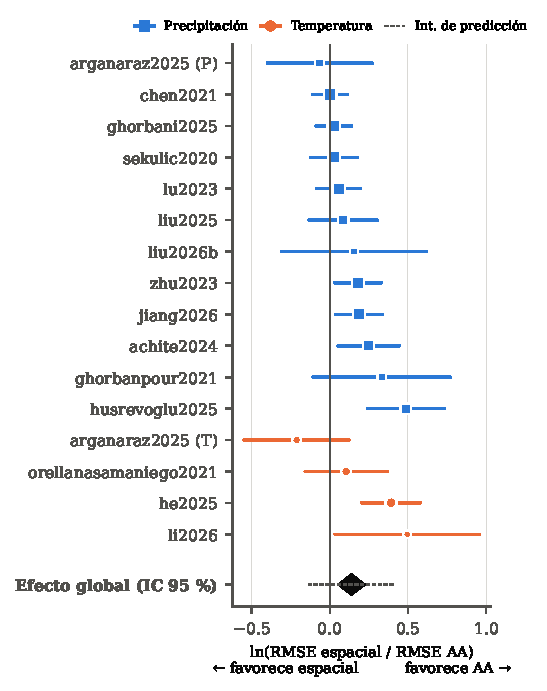
\includegraphics[width=\columnwidth]{figuras/bosque.pdf}
\caption{Gráfico de bosque de $\lnr$ por comparación, con IC~95\%. El tamaño del marcador es proporcional al peso en el modelo de efectos aleatorios. El rombo muestra el efecto global y la línea discontinua, el intervalo de predicción.}
\label{fig:bosque}
\end{figure}

\subsection{Subgrupos y sensibilidad}
La única diferencia significativa entre subgrupos fue la del esquema de validación (Tabla~\ref{tab:sub}): con estaciones independientes el efecto fue $0{,}193$, mientras que con validación cruzada fue $0{,}025$ y no significativo ($p=0{,}006$ para la diferencia). El efecto en la temperatura ($0{,}189$; $k=4$) fue mayor que en la precipitación ($0{,}118$; $k=12$), aunque muy impreciso. La ventaja del AA fue similar frente al kriging ($0{,}144$) y frente a la GWR ($0{,}119$). Cuando ambos brazos usaron las mismas covariables, el efecto fue menor ($0{,}110$) y casi homogéneo ($I^2=11\%$); cuando el AA dispuso de más información, aumentó ($0{,}243$) con heterogeneidad alta ($I^2=85\%$).

El resultado global se mantuvo al excluir los estudios con alto riesgo de sesgo ($0{,}128$; $k=13$) o la segunda comparación de Argañaraz \textit{et al.} ($0{,}151$), al incluir la comparación híbrida de Zhang \textit{et al.} ($0{,}125$; $k=17$), al usar 959 estaciones de validación para Lu \textit{et al.} ($0{,}136$), al omitir un estudio a la vez (rango $0{,}114$--$0{,}153$) y en las sensibilidades propuestas durante la extracción: sin el punto de extrapolación de Husrevoglu y Gundogdu ($0{,}120$), con el random forest espacial en Zhu \textit{et al.} ($0{,}139$) y con el SRF híbrido en Chen \textit{et al.} ($0{,}148$). También fue estable frente a la correlación supuesta entre los errores ($0{,}122$ con $\rho=0$ y $0{,}148$ con $\rho=0{,}8$), aunque la heterogeneidad estimada sí depende de ella ($I^2$ de 20 a 84\%). En cambio, en las tres comparaciones con bajo riesgo de sesgo no hubo diferencia entre los métodos ($-0{,}022$; IC~95\%: $-0{,}279$ a $0{,}236$).

\begin{table}[!t]
\caption{Análisis de subgrupos y de sensibilidad}
\label{tab:sub}
\centering
\footnotesize
\setlength{\tabcolsep}{3pt}
\begin{tabular}{@{}l r c r r@{}}
\toprule
Análisis & $k$ & $\hat{y}$ (IC 95\%) & $I^2$ (\%) & $p_{\mathrm{dif}}$\\
\midrule
Global & 16 & 0,138 (0,046; 0,231) & 60 & \\
\midrule
Precipitación & 12 & 0,118 (0,030; 0,207) & 50 & \multirow{2}{*}{0,66}\\
Temperatura & 4 & 0,189 ($-$0,299; 0,676) & 74 & \\
Kriging y variantes & 12 & 0,144 (0,016; 0,272) & 68 & \multirow{2}{*}{0,72}\\
GWR y MGWR & 4 & 0,119 ($-$0,013; 0,251) & 0 & \\
Covariables equivalentes & 11 & 0,110 (0,036; 0,184) & 11 & \multirow{2}{*}{0,25}\\
Covariables distintas & 5 & 0,243 ($-$0,064; 0,549) & 85 & \\
Estaciones independientes & 11 & 0,193 (0,060; 0,325) & 59 & \multirow{2}{*}{0,006}\\
Validación cruzada & 5 & 0,025 ($-$0,018; 0,068) & 0 & \\
\midrule
Sin riesgo alto & 13 & 0,128 (0,031; 0,226) & 54 & \\
Con el brazo híbrido (Zhang) & 17 & 0,125 (0,034; 0,216) & 61 & \\
Lu con $n=959$ & 16 & 0,136 (0,045; 0,228) & 63 & \\
Un efecto por estudio & 15 & 0,151 (0,063; 0,240) & 58 & \\
Solo riesgo bajo & 3 & $-$0,022 ($-$0,279; 0,236) & 0 & \\
$\rho = 0$ & 16 & 0,122 (0,039; 0,205) & 20 & \\
$\rho = 0{,}8$ & 16 & 0,148 (0,048; 0,248) & 84 & \\
Husrevoglu sin EMP & 16 & 0,120 (0,042; 0,197) & 48 & \\
Zhu con SRF & 16 & 0,139 (0,047; 0,232) & 60 & \\
Chen con SRF (híbrido) & 16 & 0,148 (0,060; 0,235) & 54 & \\
\bottomrule
\multicolumn{5}{@{}p{8.4cm}@{}}{$\hat{y}$: efecto combinado de $\lnr$ (REML, Hartung--Knapp). $p_{\mathrm{dif}}$: diferencia entre subgrupos.}\\
\end{tabular}
\end{table}

\subsection{Sesgo de publicación}
El gráfico de embudo no mostró una asimetría evidente (Fig.~\ref{fig:embudo}) y la prueba de Egger no fue significativa (intercepto $1{,}33$; $p=0{,}18$). Con 16 comparaciones, la potencia de esta prueba es limitada.

\begin{figure}[!t]
\centering
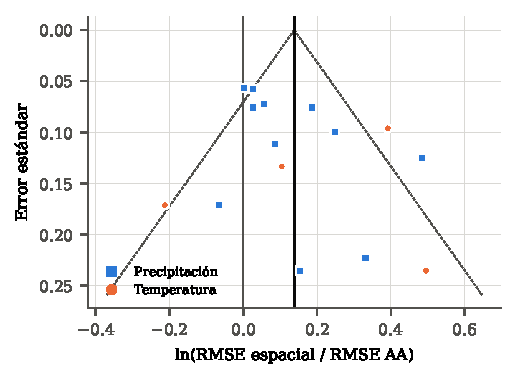
\includegraphics[width=\columnwidth]{figuras/embudo.pdf}
\caption{Gráfico de embudo. La línea vertical continua marca el efecto global y las discontinuas, los límites de confianza al 95\% en función del error estándar.}
\label{fig:embudo}
\end{figure}

\subsection{Estudios no combinados}
Dura \textit{et al.}~\cite{dura2024} compararon kriging ordinario, kriging con deriva externa (altitud y simulaciones del modelo AROME), GWR, RF y una variante RF-ratio con 3189 pluviómetros en el sur y el este de Francia. Según el KGE, los mejores modelos fueron RF-ratio, la GWR y el kriging con deriva AROME, mientras que el RF simple fue el tercero peor, por delante solo del kriging ordinario y del kriging con deriva altitudinal. Su conclusión coincide con la del metaanálisis: lo que más mejora la predicción es la covariable informativa, más que la familia del método. Del estudio de Ahmed \textit{et al.}~\cite{ahmed2026} solo se conoce que el kriging bayesiano empírico fue la mejor interpolación (RMSE de 82,49~mm frente a 87,06~mm del kriging ordinario); sin el texto completo no fue posible confirmar si XGBoost se evaluó como brazo independiente ni el número de estaciones.

\section{Discusión}

\subsection{Interpretación de los resultados}
Esta síntesis indica que, en las regiones montañosas, los modelos de AA predicen la precipitación y la temperatura con un error en promedio un 12,9\% menor que el mejor método geoestadístico. La ventaja es moderada y heterogénea: el intervalo de predicción incluye el cero y en dos comparaciones del análisis principal, más una de sensibilidad, el método espacial fue mejor. No se trata, por tanto, de una superioridad general del AA, sino de una tendencia que depende de las condiciones de cada estudio.

El factor que mejor explica esa variación es la información disponible para cada brazo. Cuando ambos usaron las mismas covariables, la ventaja del AA fue menor y casi homogénea; las mayores diferencias aparecieron cuando el kriging se aplicó solo con las estaciones y el AA dispuso de productos satelitales, reanálisis o variables del terreno~\cite{chen2021,he2025}, o la meteorología de una estación de referencia~\cite{li2026}, o cuando cada brazo usó covariables distintas~\cite{husrevoglu2025}. Esto coincide con Dura \textit{et al.}~\cite{dura2024}, para quienes la covariable AROME mejoró tanto al kriging como al RF, y con la observación de que una parte de la ventaja atribuida al AA se debe a la flexibilidad para incorporar muchas covariables más que al algoritmo en sí.

Además, la frontera entre ambas familias es cada vez más difusa. Varios estudios proponen variantes de random forest que incorporan la información espacial, en la línea de Hengl \textit{et al.}~\cite{hengl2018}: el RFSI usa las observaciones vecinas~\cite{sekulic2020} y el SRF de Chen \textit{et al.} usa la propia interpolación por kriging como covariable~\cite{chen2021}. Al tratar este último como híbrido, el kriging y el RF quedaron prácticamente empatados (35,98 frente a 35,93~mm). En Cataluña, por ejemplo, el RF estándar fue claramente peor que la regresión-kriging, y solo la variante espacial RFSI logró igualarla~\cite{sekulic2020}. La pregunta útil parece ser menos ``geoestadística o AA'' y más cómo combinar la dependencia espacial con relaciones no lineales.

\subsection{El papel de la validación}
Contra lo esperado, la ventaja del AA fue mayor con estaciones independientes que con validación cruzada, y la diferencia fue significativa. La literatura advierte que la validación cruzada aleatoria puede inflar el desempeño de los modelos flexibles cuando hay autocorrelación espacial~\cite{roberts2017,ploton2020}. En nuestro conjunto, sin embargo, casi todos los esquemas retienen estaciones completas, y los estudios con validación cruzada son los que comparan métodos con información similar. El hallazgo más relevante es que la ventaja desaparece al considerar solo los estudios con bajo riesgo de sesgo, lo que indica que depende de la calidad del diseño de validación y de la información disponible para cada brazo.

\subsection{Vacíos de evidencia}
La evidencia procede casi por completo de China e Irán, solo un estudio corresponde a los Andes~\cite{orellana2021} y ninguno al Altiplano, la región que motivó esta revisión. Tampoco se encontraron estudios elegibles de índices de sequía ni de PM2.5, y la temperatura cuenta con apenas cuatro comparaciones de resultado inconsistente. La búsqueda de verificación confirmó este vacío: hay trabajos latinoamericanos que usan AA, pero no lo comparan con un método geoestadístico validado con estaciones en montaña. El más cercano, en Costa Rica, comparó kriging ordinario y con deriva externa con random forest y Cubist para la temperatura mensual con 73 estaciones, pero es una ponencia de congreso de alcance nacional y no cumplió los criterios~\cite{mendez2020}. Los resultados no deben extrapolarse sin más a los Andes tropicales, donde la escasez de estaciones en altura es más severa que en la mayoría de los estudios incluidos.

\subsection{Limitaciones}
Primero, la varianza de cada efecto se aproximó a partir del número de estaciones de validación y de una correlación supuesta entre los errores, porque ningún estudio reportó la incertidumbre del RMSE; el efecto global fue robusto a esa suposición, pero la heterogeneidad no. Segundo, comparar el mejor método de cada familia favorece a la familia con más candidatos evaluados, que en la mayoría de los estudios fue el AA; este sesgo de selección del ganador puede haber inflado el efecto. Tercero, algunos valores se leyeron de figuras y en un caso se corrigió un error tipográfico evidente~\cite{liu2025}. Cuarto, no se consultó Web of Science, no se registró el protocolo y no se recuperó un texto completo. Por último, el número de estudios limita la potencia de los análisis de subgrupos y de la prueba de Egger.

\section{Conclusiones}
En las regiones montañosas, los modelos de aprendizaje automático predicen la precipitación y la temperatura con un error moderadamente menor que la geoestadística, pero la ventaja es heterogénea, depende de que el AA disponga de covariables más informativas y no se sostiene al considerar solo los estudios con bajo riesgo de sesgo. Para futuros estudios recomendamos comparar ambos enfoques con las mismas covariables, validar con estaciones independientes o bloques espaciales, reportar el RMSE con su número de estaciones y su incertidumbre, e incluir métodos híbridos y variantes espaciales del AA. La prioridad más clara es generar evidencia en los Andes tropicales y el Altiplano, donde esta comparación aún no se ha realizado.

\section*{Disponibilidad de datos y código}
La ficha de extracción (\texttt{datos\_extraccion.csv}), el código del metaanálisis (\texttt{metaanalisis.py}) y sus resultados están disponibles en el repositorio público \url{https://github.com/Prdelta/revisison_sistematica}, en la carpeta \texttt{articulo\_ieee/analisis}. El repositorio incluye también los criterios de elegibilidad, la ficha de extracción completa y el informe consolidado de la revisión.

\begin{thebibliography}{99}

\bibitem{viviroli2007}
D.~Viviroli, H.~H. Dürr, B.~Messerli, M.~Meybeck y R.~Weingartner, ``Mountains of the world, water towers for humanity: Typology, mapping, and global significance,'' \textit{Water Resour. Res.}, vol.~43, no.~7, art.~W07447, 2007, doi: 10.1029/2006WR005653.

\bibitem{li2011}
J.~Li y A.~D. Heap, ``A review of comparative studies of spatial interpolation methods in environmental sciences: Performance and impact factors,'' \textit{Ecol. Inform.}, vol.~6, no.~3--4, pp.~228--241, 2011, doi: 10.1016/j.ecoinf.2010.12.003.

\bibitem{appelhans2015}
T.~Appelhans, E.~Mwangomo, D.~R. Hardy, A.~Hemp y T.~Nauss, ``Evaluating machine learning approaches for the interpolation of monthly air temperature at Mt. Kilimanjaro, Tanzania,'' \textit{Spat. Stat.}, vol.~14, pp.~91--113, 2015, doi: 10.1016/j.spasta.2015.05.008.

\bibitem{hengl2018}
T.~Hengl, M.~Nussbaum, M.~N. Wright, G.~B.~M. Heuvelink y B.~Gräler, ``Random forest as a generic framework for predictive modeling of spatial and spatio-temporal variables,'' \textit{PeerJ}, vol.~6, art.~e5518, 2018, doi: 10.7717/peerj.5518.

\bibitem{sekulic2020}
A.~Sekulić, M.~Kilibarda, G.~B.~M. Heuvelink, M.~Nikolić y B.~Bajat, ``Random forest spatial interpolation,'' \textit{Remote Sens.}, vol.~12, no.~10, art.~1687, 2020, doi: 10.3390/rs12101687.

\bibitem{roberts2017}
D.~R. Roberts \textit{et al.}, ``Cross-validation strategies for data with temporal, spatial, hierarchical, or phylogenetic structure,'' \textit{Ecography}, vol.~40, no.~8, pp.~913--929, 2017, doi: 10.1111/ecog.02881.

\bibitem{ploton2020}
P.~Ploton \textit{et al.}, ``Spatial validation reveals poor predictive performance of large-scale ecological mapping models,'' \textit{Nat. Commun.}, vol.~11, art.~4540, 2020, doi: 10.1038/s41467-020-18321-y.

\bibitem{page2021}
M.~J. Page \textit{et al.}, ``The PRISMA 2020 statement: An updated guideline for reporting systematic reviews,'' \textit{BMJ}, vol.~372, art.~n71, 2021, doi: 10.1136/bmj.n71.

\bibitem{chen2021}
C.~Chen, B.~Hu y Y.~Li, ``Easy-to-use spatial random-forest-based downscaling-calibration method for producing precipitation data with high resolution and high accuracy,'' \textit{Hydrol. Earth Syst. Sci.}, vol.~25, no.~11, pp.~5667--5682, 2021, doi: 10.5194/hess-25-5667-2021.

\bibitem{ghorbanpour2021}
A.~Karbalaye Ghorbanpour, T.~Hessels, S.~Moghim y A.~Afshar, ``Comparison and assessment of spatial downscaling methods for enhancing the accuracy of satellite-based precipitation over Lake Urmia Basin,'' \textit{J. Hydrol.}, vol.~596, art.~126055, 2021, doi: 10.1016/j.jhydrol.2021.126055.

\bibitem{orellana2021}
M.~L. Orellana-Samaniego, D.~Ballari, P.~Guzman y J.~E. Ospina, ``Estimating monthly air temperature using remote sensing on a region with highly variable topography and scarce monitoring in the southern Ecuadorian Andes,'' \textit{Theor. Appl. Climatol.}, vol.~144, no.~3--4, pp.~949--966, 2021, doi: 10.1007/s00704-021-03583-3.

\bibitem{zhang2022}
J.~Zhang \textit{et al.}, ``Multi-source precipitation data merging for heavy rainfall events based on cokriging and machine learning methods,'' \textit{Remote Sens.}, vol.~14, no.~7, art.~1750, 2022, doi: 10.3390/rs14071750.

\bibitem{lu2023}
X.~Lu \textit{et al.}, ``Quantitative precipitation estimation in the Tianshan Mountains based on machine learning,'' \textit{Remote Sens.}, vol.~15, no.~16, art.~3962, 2023, doi: 10.3390/rs15163962.

\bibitem{zhu2023}
H.~Zhu, H.~Liu, Q.~Zhou y A.~Cui, ``Towards an accurate and reliable downscaling scheme for high-spatial-resolution precipitation data,'' \textit{Remote Sens.}, vol.~15, no.~10, art.~2640, 2023, doi: 10.3390/rs15102640.

\bibitem{achite2024}
M.~Achite, P.~Tsangaratos, G.~Pellicone, B.~Mohammadi y T.~Caloiero, ``Application of multiple spatial interpolation approaches to annual rainfall data in the Wadi Cheliff basin (north Algeria),'' \textit{Ain Shams Eng. J.}, vol.~15, no.~3, art.~102578, 2024, doi: 10.1016/j.asej.2023.102578.

\bibitem{dura2024}
V.~Dura, G.~Evin, A.-C. Favre y D.~Penot, ``Spatial interpolation of seasonal precipitations using rain gauge data and convection-permitting regional climate model simulations in a complex topographical region,'' \textit{Int. J. Climatol.}, vol.~44, no.~16, pp.~5745--5760, 2024, doi: 10.1002/joc.8662.

\bibitem{arganaraz2025}
C.~I. Argañaraz, A.~Salcedo-Bosch, S.~Lolli y G.~Curci, ``Building a high-resolution climate gridded dataset in complex terrain: Validating different methods in the Abruzzo region in Italy,'' \textit{Int. J. Climatol.}, vol.~45, no.~16, art.~e70153, 2025, doi: 10.1002/joc.70153.

\bibitem{ghorbani2025}
K.~Ghorbani, M.~Salarijazi, L.~R. Ghaleh y E.~Valizadeh, ``Improve precipitation zoning accuracy by applying ensemble learning models based on interpolation and data mining integration,'' \textit{Water Resour. Manage.}, vol.~39, no.~7, pp.~3149--3171, 2025, doi: 10.1007/s11269-025-04101-0.

\bibitem{he2025}
Y.~He \textit{et al.}, ``Distributed modeling for daily mean air temperature of Fujian Province under rugged terrain with different land surface types,'' \textit{IEEE J. Sel. Topics Appl. Earth Observ. Remote Sens.}, vol.~18, pp.~26908--26923, 2025, doi: 10.1109/JSTARS.2025.3622347.

\bibitem{husrevoglu2025}
M.~Husrevoglu y I.~B. Gundogdu, ``Evaluating the performance of ANN and ANFIS models for spatial precipitation prediction in complex terrain: A case study in central Anatolia,'' \textit{Theor. Appl. Climatol.}, vol.~156, no.~7, art.~395, 2025, doi: 10.1007/s00704-025-05637-2.

\bibitem{liu2025}
J.~Liu \textit{et al.}, ``Comparative study on the different downscaling methods for GPM products in complex terrain areas,'' \textit{Earth}, vol.~6, no.~4, art.~129, 2025, doi: 10.3390/earth6040129.

\bibitem{ahmed2026}
P.~B.~S. Ahmed, N.~F. Mustafa y M.~H.~M. Baban, ``Enhanced spatial precipitation maps by integrating XGBoost machine learning, terrain indices, and optimal interpolation,'' \textit{Theor. Appl. Climatol.}, vol.~157, no.~5, art.~270, 2026, doi: 10.1007/s00704-026-06177-z.

\bibitem{jiang2026}
L.~Jiang \textit{et al.}, ``Comparative analysis of spatial interpolation methods for daily rainfall data in complex terrain,'' \textit{Theor. Appl. Climatol.}, vol.~157, no.~3, art.~130, 2026, doi: 10.1007/s00704-026-06041-0.

\bibitem{liu2026}
L.~Liu \textit{et al.}, ``A spatiotemporal interpolation method for regional precipitation data based on a spatiotemporal decay graph model,'' \textit{Climate}, vol.~14, no.~7, art.~136, 2026, doi: 10.3390/cli14070136.

\bibitem{li2026}
S.~Li \textit{et al.}, ``High-precision spatial interpolation of meteorological variables in complex terrain using machine learning methods,'' \textit{Sensors}, vol.~26, no.~7, art.~2167, 2026, doi: 10.3390/s26072167.

\bibitem{hedges1999}
L.~V. Hedges, J.~Gurevitch y P.~S. Curtis, ``The meta-analysis of response ratios in experimental ecology,'' \textit{Ecology}, vol.~80, no.~4, pp.~1150--1156, 1999, doi: 10.1890/0012-9658(1999)080[1150:TMAORR]2.0.CO;2.

\bibitem{viechtbauer2005}
W.~Viechtbauer, ``Bias and efficiency of meta-analytic variance estimators in the random-effects model,'' \textit{J. Educ. Behav. Stat.}, vol.~30, no.~3, pp.~261--293, 2005, doi: 10.3102/10769986030003261.

\bibitem{hartung2001}
J.~Hartung y G.~Knapp, ``A refined method for the meta-analysis of controlled clinical trials with binary outcome,'' \textit{Stat. Med.}, vol.~20, no.~24, pp.~3875--3889, 2001, doi: 10.1002/sim.1009.

\bibitem{higgins2002}
J.~P.~T. Higgins y S.~G. Thompson, ``Quantifying heterogeneity in a meta-analysis,'' \textit{Stat. Med.}, vol.~21, no.~11, pp.~1539--1558, 2002, doi: 10.1002/sim.1186.

\bibitem{egger1997}
M.~Egger, G.~Davey Smith, M.~Schneider y C.~Minder, ``Bias in meta-analysis detected by a simple, graphical test,'' \textit{BMJ}, vol.~315, no.~7109, pp.~629--634, 1997, doi: 10.1136/bmj.315.7109.629.

\bibitem{wolff2019}
R.~F. Wolff \textit{et al.}, ``PROBAST: A tool to assess the risk of bias and applicability of prediction model studies,'' \textit{Ann. Intern. Med.}, vol.~170, no.~1, pp.~51--58, 2019, doi: 10.7326/M18-1376.

\bibitem{mendez2020}
M.~Méndez y L.~A. Calvo-Valverde, ``Comparison performance of machine learning and geostatistical methods for the interpolation of monthly air temperature over Costa Rica,'' \textit{IOP Conf. Ser.: Earth Environ. Sci.}, vol.~432, art.~012011, 2020, doi: 10.1088/1755-1315/432/1/012011.

\end{thebibliography}

\end{document}
